\begin{titlepage}
%\begin{center}
\begin{center}
% 	%\textsc{\Large Spatiotemporal modeling of fuelwood environmental impacts: towards improved accounting for non-renewable biomass}\\[0.5cm]
% 	\textsc{\Large Explorador de cambio clim\'atico y Biodiversidad}\\[0.5cm]

% 	%\textsc{\Large Mofuss: Modeling fuelwood savings scenarios - version 1.0}\\[0.25cm]
% 	\textsc{\Large Comisi\'on Nacional para el Conocimiento y Uso de la Biodiversidad (CONABIO)}\\[0.25cm]


% \HRule \\[0.25cm]
% 	{\huge\textbf{Reporte de areas seleccionadas \\}}
% \HRule \\[0.25cm]
	
% 	\emph{{\large Este es un reporte generado autom\'aticamente que resume la consulta realizada en el explorador de cambio clim\'atico y biodiversidad. \\}}

% 	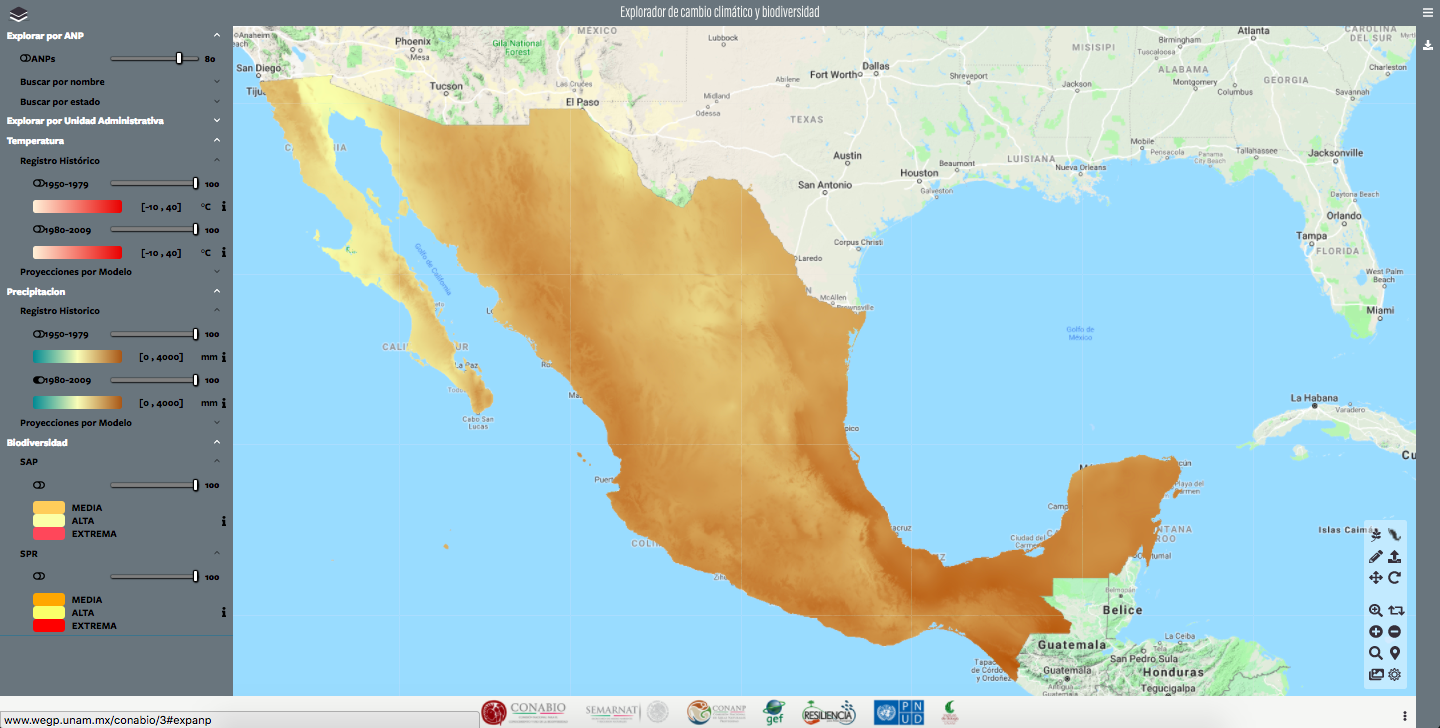
\includegraphics[width=0.9\linewidth]{./logos/entry.png} \\

% 	\textbf{Proyecto financiado por: } \\

	\begin{table}[h!]
	\centering
		%\begin{center}
			\begin{tabular}{ccccc}

				%\multicolumn{3}{c}{
\includegraphics[width=6cm]{./logos/conabio.png}} \\ 
				%
\includegraphics[width=4cm]{./logos/semarnat.png} &
				%
\includegraphics[width=4cm]{./logos/conanp.png} &
				%
\includegraphics[height=2.5cm]{./logos/gef.png} \\

				%
\includegraphics[width=4cm]{./logos/resiliencia.png} &
				%
\includegraphics[width=4cm]{./logos/pnud.png} &
				%
\includegraphics[height=2.5cm]{./logos/unam.png}


				
\includegraphics[width=3cm]{./logos/conabio.png} &
				
\includegraphics[height=2.5cm]{./logos/unam.png} &
				
\includegraphics[width=3cm]{./logos/semarnat.png} &
				
\includegraphics[width=3cm]{./logos/conanp.png} &
				
\includegraphics[width=3cm]{./logos/logoINECC.png} \\

				\multicolumn{2}{c}{
\includegraphics[height=2.5cm]{./logos/gef.png}} &
				\multicolumn{2}{c}{
\includegraphics[width=3cm]{./logos/resiliencia.png}} &
				
\includegraphics[width=3cm]{./logos/pnud.png}


			\end{tabular}
		%\begin{center}
	\end{table}
	\bigskip
	\bigskip
	\large\textbf{EXPLORADOR DE CAMBIO CLIM\'ATICO Y BIODIVERSIDAD }\\
	\bigskip
	COMISI\'ON NACIONAL PARA EL CONOCIMIENTO Y USO DE LA BIODIVERSIDAD \\
	(CONABIO) \\

	\textbf{Reporte de \'Areas Seleccionadas} \\
	Este es un reporte generado autom\'aticamente que resume la consulta generada en el explorador de cambio clim\'atico y biodiversidad
	\bigskip
	\bigskip
	\bigskip
	%\small{Conabio, IB-UNAM, Conanp, PNUD, INECC, Reporte de \'areas seleccionadas. Explorador de cambio clim\'atico y biodiversidad. Comisi\'on Nacional para el Conocimiento y Uso de la Biodiversidad, en \ref{http://www.biodiversidad.gob.mx/pais/cambio_climatico.html} Fecha de consulta: }
	%\pagebreak

\end{center}

% \HRule \\[0.25cm]
% { 
% 	\huge \bfseries Summary Report for %\input{../LULCC/TempTables/Country.txt}}
% }
% \HRule \\[0.25cm]
% {
% 	\emph{\large This is an automated report generated by The present document summarizes main results of the model for the red polygon in the map shown here below.\\ } 
% }


% %\includegraphics[width=0.9\linewidth]{../OutBaU/png/Area_of_Interest}

% \textbf{Project funded by:}\\
% %\includegraphics[width=0.2\linewidth]{../LULCC/Wizard_imgs/GACC}
% \end{center}


% \pagebreak 
% %\setlength{\parindent}{0cm}

% \begin{flushleft}

% %A. Ghilardi, R. Bailis, J-F. Mas, R. Drigo, O. Masera. \textbf{Summary Report for \input{../LULCC/TempTables/Country.txt}}- Spatiotemporal modeling of fuelwood environmental impacts. \the\year. CIGA-UNAM and SEI-US. \pageref{lastpage} p.
% \bigskip

\begin{flushleft}
\small{Conabio, IB-UNAM, Conanp, PNUD, INECC, Reporte de \'areas seleccionadas. Explorador de cambio clim\'atico y biodiversidad. Comisi\'on Nacional para el Conocimiento y Uso de la Biodiversidad, en \url{http://www.biodiversidad.gob.mx/pais/cambio_climatico.html} Fecha de consulta: \input{fecha.txt}}
% Comisi\'on Nacional para el Conocimiento y Uso de la Biodiversidad (CONABIO) \\
% Liga Perif\'erico - Insurgentes Sur 4903, \\
% Parques del Pedregal, Del. Tlalpan, \\
% Ciudad de M\'exico. C.P. 14010 \\
% Tel: 5004.5000 \\
% Web: www.gob.mx/conabio
\bigskip
\end{flushleft}

% Centro de Investigaciones en Geografía Ambiental \\
% Universidad Nacional Autónoma de México \\
% Antigua carretera a Pátzcuaro 8701, \\
% Col. Exhacienda de San José de la Huerta, \\
% Morelia, Michoacán, C.P. 58190, Mexico. \\
% Tel: +52 443-322-3854 \\
% Web: www.ciga.unam.mx
% \bigskip

% Stockholm Environment Institute - US Centre \\
% 11 Curtis Ave, \\
% Somerville, MA 02144, United States. \\
% Phone: +1 617-627-3786 \\
% Web: www.sei-us.org
% \bigskip

% Author contact: Adrian Ghilardi, \\
% Centro de Investigaciones en Geografía Ambiental, \\
% Universidad Nacional Autónoma de México. \\
% aghilardi@ciga.unam.mx
% \bigskip \bigskip \bigskip \bigskip \bigskip \bigskip \bigskip \bigskip

% %Cover Photo: Cow dung drying in Haryana, Northern India, for
% %use as a domestic energy source amongst rural households.
% %© Adrian Ghilardi
% %\\[3.0cm]

% This publication may be reproduced in whole or in part and in any
% form for educational or non-profit purposes, without special permission
% from the copyright holder(s) provided acknowledgement
% of the source is made. No use of this publication may be made for
% resale or other commercial purpose, without the written permission
% of the copyright holder(s).
% \bigskip


% %\includegraphics[width=0.1\linewidth]{../LULCC/Wizard_imgs/SEI}

% \end{flushleft}
\end{titlepage}